\section{Experiments}
\label{sec:feats_results}
In this section, we first lead preliminary experiments where we qualitatively study the behaviour of our autoencoder method through the inspection of the activation maps at the bottleneck layer.
Next, we quantify the added value of our data augmentation strategy.
Also, we experiment on the effect of padding strategies, namely the zero padding and symmetric padding, and assess their discrepancies in performance on a Brain sequence.
The proposed feature extraction methods are then quantitively compared and ranked.


\subsection{Activation Maps} \label{ch:act_maps}
Visualizing the filter responses of a \gls{cnn} allows to get some insight into what the network actually ``sees'' and ``focuses'' on in its learning task.
In particular, we consider the activation maps of the layer where our features are extracted, i.e. the last ReLU of the deepest layer.
We randomly sampled an image, performed a forward pass on a trained \textit{U-Net AE} model, and visualized $11$ out of the $512$ activation maps.
Fig. \ref{fig:activatiom_maps} shows examples on a Brain and Slitlamp sequence,

\begin{figure}[!htbp]
  \centering
  \subfloat[Example on Brain]
  {
    \label{fig:subfig:activatiom_map_ds09}
    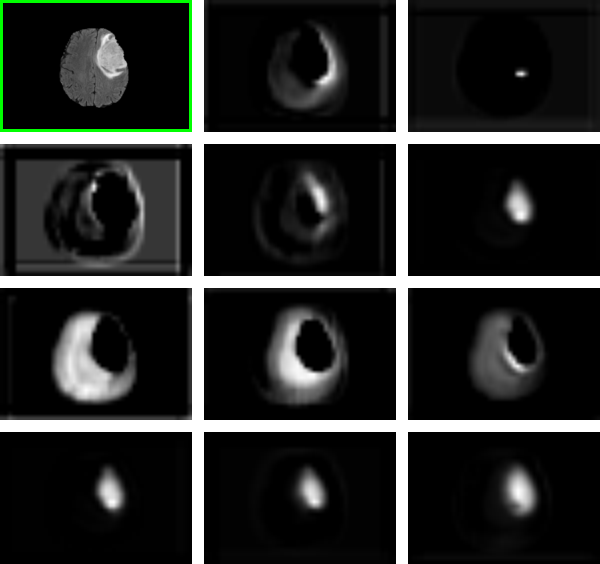
\includegraphics[height=6.2cm]{activation_maps/activations_ds09_0097}
  }
  \hfill
  \subfloat[Example on Slitlamp]
  {
    \label{fig:subfig:activatiom_map_ds13}
    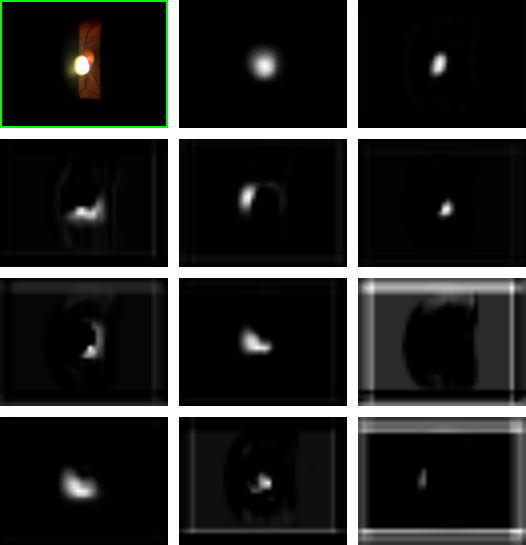
\includegraphics[height=6.2cm]{activation_maps/activations_ds13_0109}
  }
  \caption[Activation maps]{Activation maps of the \textit{U-Net AE} model for Brain and Slitlamp images.
    The input image is at the upper-left.
    The other plots show randomly chosen activation maps extracted at the bottleneck layer.}
  \label{fig:activatiom_maps}
\end{figure}

\subsection{Data Augmentation} \label{ch:nec_data_gen}
To explore the importance of data augmentation, we trained the \textit{U-Net AE} model both with and without data augmentation.
As for all experiments, we performed the training and evaluation with ten repetitions, then took the mean \textit{max F1-Score}.
We performed this experiment on one dataset per image modality.
The results are summarized in Tab. \ref{tab:data_gen_nec}.
\vspace{30pt}

\begin{table}[!htbp]
   \centering
   \caption[Importance of data generator]{Influence of data augmentation in terms of mean \textit{max F1-Score} over ten training repetitions.
     A \textit{U-Net AE} model is trained with and without data agumentation.}
   \begin{tabular}{l|*{4}{c|}}
      \toprule
       & \rotatebox[origin=cB]{90}{\parbox[t]{3.2cm}{\hspace{3pt} \textbf{Tweezer} \hspace*{\fill}}}
       & \rotatebox[origin=cB]{90}{\parbox[t]{3.2cm}{\hspace{3pt} \textbf{Brain} \hspace*{\fill}}}
       & \rotatebox[origin=cB]{90}{\parbox[t]{3.2cm}{\hspace{3pt} \textbf{Cochlea} \hspace*{\fill}}}
       & \rotatebox[origin=cB]{90}{\parbox[t]{3.2cm}{\hspace{3pt} \textbf{Slitlamp} \hspace*{\fill}}} \\
      \midrule
      Without data augmentation & 0.9826 & 0.9792 & 0.9587 & 0.9800 \\\midrule
      With data augmentation & 0.9832 & 0.9810 & 0.9621 & 0.9863 \\\midrule\midrule
      Improvement & \textbf{0.061\%} & \textbf{0.184\%} & \textbf{0.355\%} & \textbf{0.643\%} \\
      \bottomrule
   \end{tabular}
   \label{tab:data_gen_nec}
\end{table}

\subsection{Zero-Padding vs. Symmetric-Padding} \label{ch:zero_vs_sym_pad}
As convolutional operations are only valid on a neighborhood whose size matches the kernel size, one typically resorts to zero-padding.
In particular, we add to the input tensor zero-values at its borders so as to conserve the same size at the output.
Another strategy is to perform symmetric-padding, where we add rows and columns of pixels according to a mirror reflection of the input.
To investigate the influence of the border-effect due to zero-padding, we evaluate the \textit{U-Net Pred Loc} model using symmetric-padding on all convolutional layers.
We trained the model on one dataset per image modality.
Fig. \ref{fig:activatiom_maps_sym} shows example activation maps at the bottleneck on a Brain sequence.

\begin{figure}[!htbp]
  \centering
  \subfloat[Activation maps with zero-padding]
  {
    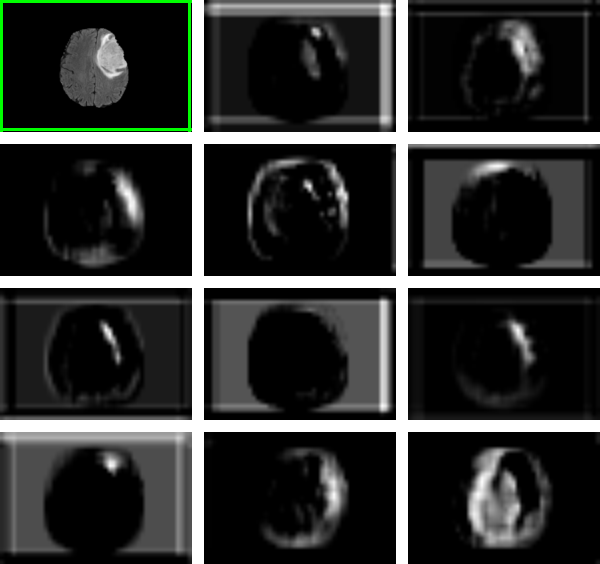
\includegraphics[height=5.8cm]{activation_maps/activations_ds09_0097_gaze_rec}
  }
  \hfill
  \subfloat[Activation maps with symmetric-padding]
  {
    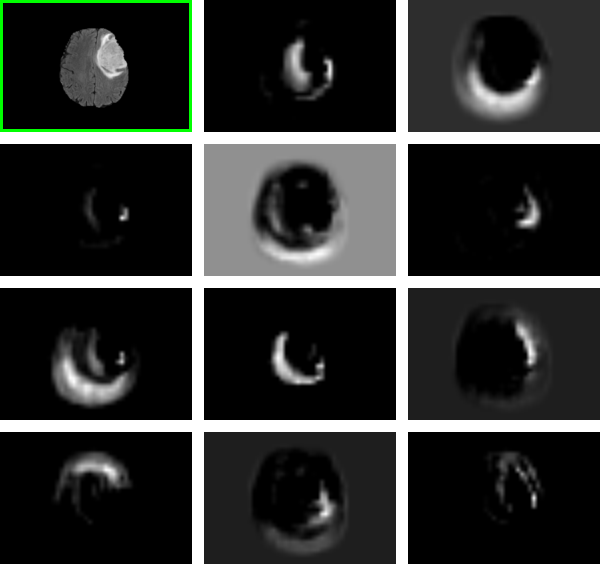
\includegraphics[height=5.8cm]{activation_maps/activations_ds09_0097_gaze_rec_sympadded}
  }
  \caption[Activation maps symmetric padding]{Activation maps of a \textit{U-Net Prior AE} model with (a) zero-padding (standard configuration) and (b) symmetric-padding for the convolutional layers.
    The upper left image shows an input image from the Brain dataset.
    The other plots show some randomly chosen activation maps.}
  \label{fig:activatiom_maps_sym}
\end{figure}

Next, we quantify the discrepancies in performance by taking a single sequence of each type.
Tab. \ref{tab:zero_vs_sym_padd} shows the mean \textit{max F1-Scores} over ten repetitions using zero-padding and symmetric-padding.

\begin{table}[!htbp]
   \centering
   \caption[Zero-padding vs. symmetric-padding]{Comparison of zero-padding vs. symmetric-padding using \textit{U-Net Prior AE} model.
     We give the mean \textit{max F1-Scores} for one dataset per image modality over ten repetitions.
     The last column indicates the improvement due to symmetric-padding.}
   \small
   \begin{tabular}{l|c|c||c|}
      \toprule
       & \Gape[6pt][6pt]{\rotatebox[origin=cB]{90}{\parbox[t]{2.6cm}{U-Net Prior AE \\ \textit{\textbf{Zero-Pad}\hspace*{\fill}}}}}
       & \rotatebox[origin=cB]{90}{\parbox[t]{2.6cm}{U-Net Prior AE \\ \textit{\textbf{Symmetric-Pad}\hspace*{\fill}}}}
       & \rotatebox[origin=cB]{90}{\parbox[t]{2.6cm}{\textbf{Improvement\hspace*{\fill}}}} \\
      \midrule
      \textbf{Tweezer} & 0.9832 & 0.9823  & \textbf{-0.091\%} \\\midrule
      \textbf{Brain} & 0.9810 & 0.9830 &  \textbf{+0.203\%} \\\midrule
%      {\scriptsize MRI Brain B} & \scriptsize 0.9292 & \scriptsize 0.9278 & \scriptsize -0.0014 \\\midrule
%      {\scriptsize MRI Brain C} & \scriptsize 0.9742 & \scriptsize 0.9760 & \scriptsize +0.0018 \\\midrule
%      {\scriptsize MRI Brain D} & \scriptsize 0.9463 & \scriptsize 0.9470 & \scriptsize +0.0006 \\\midrule
%      {\scriptsize MRI Brain (B-D)} & \scriptsize 0.9463 & \scriptsize 0.9431 & \scriptsize -0.0032 \\\midrule\midrule
      \textbf{Cochlea} & 0.9621 & 0.9535 & \textbf{-0.893\%} \\\midrule
%      {\scriptsize CT Inner Ear B} & \scriptsize 0.9623 & \scriptsize 0.9566 & \scriptsize -0.0057 \\\midrule\midrule
      \textbf{Slitlamp} & 0.9863 & 0.9860 & \textbf{-0.03\%} \\
%      {\scriptsize Slit-Lamp B} & \scriptsize 0.9747 & \scriptsize 0.9796 & \scriptsize +0.0049 \\\midrule
%      {\scriptsize Slit-Lamp C} & \scriptsize 0.9826 & \scriptsize 0.9846 & \scriptsize +0.002 \\\midrule
%      {\scriptsize Slit-Lamp D} & \scriptsize 0.9852 & \scriptsize 0.9886 & \scriptsize +0.0034 \\\midrule
%      {\scriptsize Slit-Lamp A-D} & \scriptsize 0.9785 & \scriptsize 0.9763 & \scriptsize -0.0022 \\
      \bottomrule
   \end{tabular}
   \label{tab:zero_vs_sym_padd}
\end{table}

\subsection{Quantitative study and PR curves}
The Brain and Slitlamp sequences are divided into $4$ scans/videos, which we refer to with letters A to D.
the Cochlea sequences are divided into $2$ scans, which we refer to with letters A and B.
The Tweezer type is a single video.
For each sequence/type and method, we perform a two-sided Welch's t-test \cite{welch47} to determine whether the score reached by the individual method is significantly different to the score reached by the best method for that dataset/sequence.
Tab. \ref{tab:final_results} gives the performances for each dataset/sequence and method in terms of \textit{max F1-Scores} averaged over ten repetitions.
All values marked in bold font are not significantly different to the best score for a significance level of $0.05$.
The last row shows how many times the given method did not significantly perform worse than the best method.
We name this score \textit{Top-Sig-Score}.
All best scores per dataset are in red.

Next, we visualize the PR curves of the proposed methods on two sequences.
Fig. \ref{fig:curves_ds14} and \ref{fig:curves_ds16} shows the PR curves and  \textit{max F1-scores} on a Brain and Slitlamp sequence, respectively.

\begin{table}[!htbp]
   \centering
   \caption[Feature quality]{Performance in terms of \textit{max F1-Scores} averaged over ten repetitions for each dataset and method, respectively. The according standard deviation is given underneath each score. Best scores per dataset are marked in red font. All bold marked scores are not significantly different from the best score when testing by a two-sided Welch's t-test with a significance level of 0.05. The last row shows on how many datasets the specific method was not significantly different to the best method.}
   \begin{tabular}{l|*{9}{c|}}
      \toprule
       & \rotatebox[origin=cB]{90}{\parbox[t]{4cm}{BoVW \hspace*{\fill}}} 
       & \rotatebox[origin=cB]{90}{\parbox[t]{4cm}{ScSP \hspace*{\fill}}} 
       & \rotatebox[origin=cB]{90}{\parbox[t]{4cm}{VGG \hspace*{\fill}}} 
       & \rotatebox[origin=cB]{90}{\parbox[t]{4cm}{U-Net AE \hspace*{\fill}}}
       & \rotatebox[origin=cB]{90}{\parbox[t]{4cm}{U-Net Prior AE \hspace*{\fill}}}
       & \rotatebox[origin=cB]{90}{\parbox[t]{4cm}{U-Net Pred Loc \hspace*{\fill}}}
       & \rotatebox[origin=cB]{90}{\parbox[t]{4cm}{U-Net Pred Loc Frozen \hspace*{\fill}}}
       & \rotatebox[origin=cB]{90}{\parbox[t]{4cm}{U-Net Motion Pred \hspace*{\fill}}}
       & \rotatebox[origin=cB]{90}{\parbox[t]{4cm}{U-Net Motion Pred LSTM \hspace*{\fill}}}  \\
       & \raisebox{-\totalheight}{
\includegraphics[width=0.8cm]{icons/bovw}} 
       & \raisebox{-\totalheight}{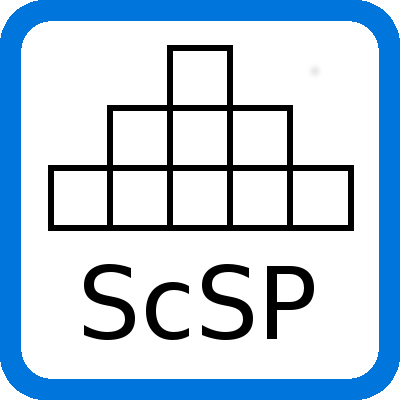
\includegraphics[width=0.8cm]{icons/scsp}} 
       & \raisebox{-\totalheight}{
\includegraphics[width=0.8cm]{icons/vgg}} 
       & \raisebox{-\totalheight}{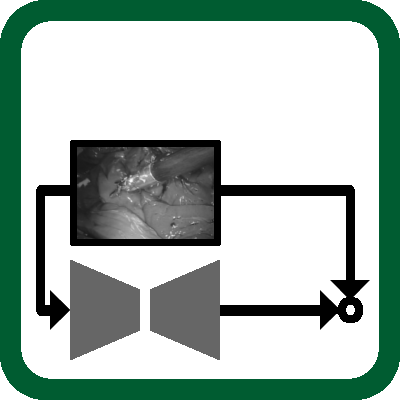
\includegraphics[width=0.8cm]{icons/unet_rec}} 
       & \raisebox{-\totalheight}{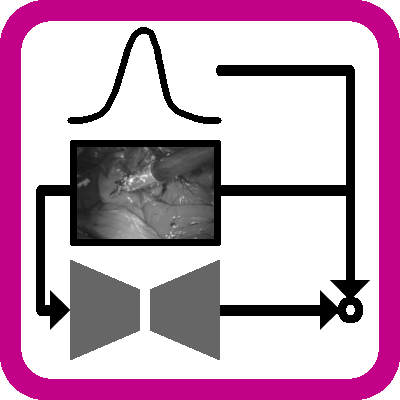
\includegraphics[width=0.8cm]{icons/unet_gaze_rec}} 
       & \raisebox{-\totalheight}{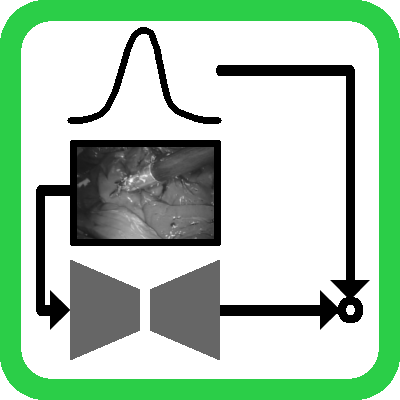
\includegraphics[width=0.8cm]{icons/unet_gaze_prob}} 
       & \raisebox{-\totalheight}{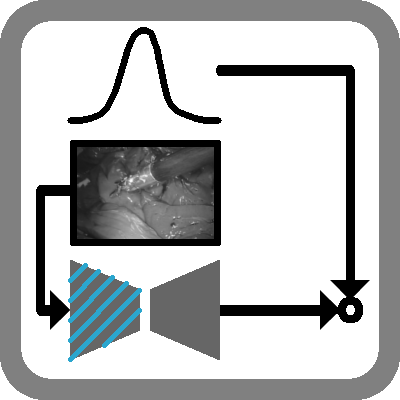
\includegraphics[width=0.8cm]{icons/unet_gaze_prob_freeze}} 
       & \raisebox{-\totalheight}{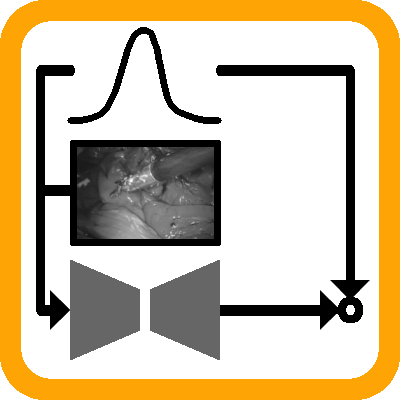
\includegraphics[width=0.8cm]{icons/unet_gaze_prob_concat}} 
       & \raisebox{-\totalheight}{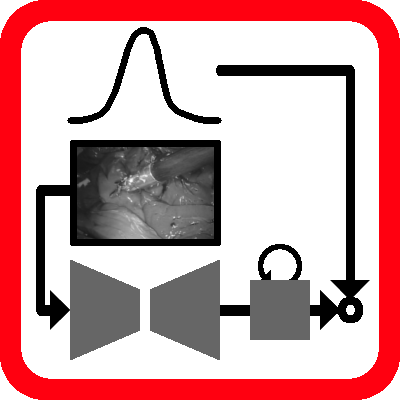
\includegraphics[width=0.8cm]{icons/unet_gaze_prob_lstm}}\\
      \midrule\midrule
      {\scriptsize Tweezer} & \scriptsize 0.6649 & \scriptsize 0.8998 & \scriptsize 0.9647 & \textbf{\scriptsize 0.9830} & {\color{red} \textbf{\scriptsize 0.9832}} & \scriptsize 0.9791 & \scriptsize 0.9811 & \scriptsize 0.9776 & \scriptsize 0.9807 \\[-4pt]
       & \tiny $\pm$6.24e-4 & \tiny $\pm$6.04e-4 & \tiny $\pm$3.87e-4 & \tiny $\pm$4.84e-4 & \tiny $\pm$4.22e-4 & \tiny $\pm$1.84e-3 & \tiny $\pm$4.78e-4 & \tiny $\pm$2.93e-3 & \tiny $\pm$7.21e-4 \\\midrule\midrule
      {\scriptsize Brain A} & \scriptsize 0.3163 & \scriptsize 0.9288 & \scriptsize 0.9666 & \textbf{\scriptsize 0.9774} & {\color{red} \textbf{\scriptsize 0.9810}} & \scriptsize 0.9764 & \textbf{\scriptsize 0.9806} & \scriptsize 0.9673 & \textbf{\scriptsize 0.9794} \\[-4pt]
       & \tiny $\pm$3.61e-3 & \tiny $\pm$5.05e-3 & \tiny $\pm$2.10e-3 & \tiny $\pm$4.65e-3 & \tiny $\pm$3.95e-3 & \tiny $\pm$3.30e-3 & \tiny $\pm$3.28e-3 & \tiny $\pm$8.90e-3 & \tiny $\pm$5.02e-3 \\\midrule
      {\scriptsize Brain B} & \scriptsize 0.7502 & \scriptsize 0.8568 & \scriptsize 0.8911 & \textbf{\scriptsize 0.9232} & \textbf{\scriptsize 0.9292} & \scriptsize 0.9142 & \textbf{\scriptsize 0.9253} & {\color{red} \textbf{\scriptsize 0.9297}} & \scriptsize 0.9201 \\[-4pt]
       & \tiny $\pm$8.20e-3 & \tiny $\pm$7.36e-3 & \tiny $\pm$3.88e-3 & \tiny $\pm$5.63e-3 & \tiny $\pm$3.74e-3 & \tiny $\pm$8.59e-3 & \tiny $\pm$4.83e-3 & \tiny $\pm$7.09e-3 & \tiny $\pm$7.90e-3 \\\midrule
      {\scriptsize Brain C} & \scriptsize 0.7911 & \scriptsize 0.8957 & \scriptsize 0.9345 & \textbf{\scriptsize 0.9766} & \textbf{\scriptsize 0.9742} & \scriptsize 0.9695 & {\color{red} \textbf{\scriptsize 0.9774}} & \textbf{\scriptsize 0.9742} & \scriptsize 0.9729 \\[-4pt]
       & \tiny $\pm$7.21e-3 & \tiny $\pm$2.66e-3 & \tiny $\pm$3.28e-3 & \tiny $\pm$3.75e-3 & \tiny $\pm$3.31e-3 & \tiny $\pm$2.96e-3 & \tiny $\pm$2.11e-3 & \tiny $\pm$5.15e-3 & \tiny $\pm$4.03e-3 \\\midrule
      {\scriptsize Brain D} & \scriptsize 0.7035 & \scriptsize 0.7764 & \scriptsize 0.8548 & {\color{red} \textbf{\scriptsize 0.9470}} & \textbf{\scriptsize 0.9463} & \scriptsize 0.9207 & \scriptsize 0.9247 & \scriptsize 0.9293 & \scriptsize 0.9276 \\[-4pt]
       & \tiny $\pm$1.27e-2 & \tiny $\pm$6.67e-3 & \tiny $\pm$6.11e-3 & \tiny $\pm$5.42e-3 & \tiny $\pm$4.67e-3 & \tiny $\pm$5.48e-3 & \tiny $\pm$5.48e-3 & \tiny $\pm$4.51e-3 & \tiny $\pm$5.00e-3 \\\midrule
      {\scriptsize Brain (B-D)} & \scriptsize 0.6753 & \scriptsize 0.8046 & \scriptsize 0.8640 & {\color{red} \textbf{\scriptsize 0.9482}} & \textbf{\scriptsize 0.9463} & \scriptsize 0.9167 & \scriptsize 0.9399 & \scriptsize 0.9236 & \scriptsize 0.9310 \\[-4pt]
       & \tiny $\pm$4.83e-3 & \tiny $\pm$1.67e-3 & \tiny $\pm$2.61e-3 & \tiny $\pm$4.65e-3 & \tiny $\pm$3.80e-3 & \tiny $\pm$1.30e-2 & \tiny $\pm$3.40e-3 & \tiny $\pm$5.42e-3 & \tiny $\pm$1.16e-2 \\\midrule\midrule
      {\scriptsize Cochlea A} & \scriptsize 0.5527 & \scriptsize 0.8680 & \scriptsize 0.7400 & \textbf{\scriptsize 0.9624} & \textbf{\scriptsize 0.9621} & \scriptsize 0.9565 & \scriptsize 0.9554 & \textbf{\scriptsize 0.9660} & {\color{red} \textbf{\scriptsize 0.9686}} \\[-4pt]
       & \tiny $\pm$1.24e-2 & \tiny $\pm$1.02e-2 & \tiny $\pm$6.09e-3 & \tiny $\pm$4.75e-3 & \tiny $\pm$6.38e-3 & \tiny $\pm$8.60e-3 & \tiny $\pm$6.42e-3 & \tiny $\pm$7.20e-3 & \tiny $\pm$8.12e-3 \\\midrule
      {\scriptsize Cochlea B} & \scriptsize 0.4659 & \scriptsize 0.8372 & \scriptsize 0.7786 & {\color{red} \textbf{\scriptsize 0.9628}} & \textbf{\scriptsize 0.9623} & \scriptsize 0.9481 & \scriptsize 0.9443 & \scriptsize 0.9560 & \scriptsize 0.9476 \\[-4pt]
       & \tiny $\pm$1.78e-2 & \tiny $\pm$5.55e-3 & \tiny $\pm$5.11e-3 & \tiny $\pm$3.34e-3 & \tiny $\pm$1.41e-3 & \tiny $\pm$7.64e-3 & \tiny $\pm$6.63e-3 & \tiny $\pm$4.61e-3 & \tiny $\pm$1.35e-2 \\\midrule\midrule
      {\scriptsize Slitlamp A} & \scriptsize 0.8912 & \scriptsize 0.9742 & \scriptsize 0.9784 & \textbf{\scriptsize 0.9845} & \textbf{\scriptsize 0.9863} & \scriptsize 0.9839 & {\color{red} \textbf{\scriptsize 0.9890}} & \scriptsize 0.9788 & \scriptsize 0.9780 \\[-4pt]
       & \tiny $\pm$9.97e-3 & \tiny $\pm$5.34e-3 & \tiny $\pm$3.57e-3 & \tiny $\pm$5.20e-3 & \tiny $\pm$3.36e-3 & \tiny $\pm$4.06e-3 & \tiny $\pm$2.74e-3 & \tiny $\pm$8.12e-3 & \tiny $\pm$4.20e-3 \\\midrule
      {\scriptsize Slitlamp B} & \scriptsize 0.6454 & \textbf{\scriptsize 0.9909} & \scriptsize 0.9775 & \scriptsize 0.9687 & \scriptsize 0.9747 & \textbf{\scriptsize 0.9888} & \scriptsize 0.9707 & {\color{red} \textbf{\scriptsize 0.9913}} & \scriptsize 0.9827 \\[-4pt]
       & \tiny $\pm$1.29e-2 & \tiny $\pm$2.48e-3 & \tiny $\pm$4.05e-3 & \tiny $\pm$8.44e-3 & \tiny $\pm$6.62e-3 & \tiny $\pm$4.32e-3 & \tiny $\pm$5.33e-3 & \tiny $\pm$2.43e-3 & \tiny $\pm$4.05e-3 \\\midrule
      {\scriptsize Slitlamp C} & \scriptsize 0.8681 & {\color{red} \textbf{\scriptsize 0.9870}} & \scriptsize 0.9724 & \textbf{\scriptsize 0.9862} & \textbf{\scriptsize 0.9826} & \scriptsize 0.9686 & \textbf{\scriptsize 0.9792} & \scriptsize 0.9736 & \scriptsize 0.9707 \\[-4pt]
       & \tiny $\pm$5.63e-3 & \tiny $\pm$3.43e-3 & \tiny $\pm$4.55e-3 & \tiny $\pm$7.43e-3 & \tiny $\pm$5.50e-3 & \tiny $\pm$1.33e-2 & \tiny $\pm$8.54e-3 & \tiny $\pm$9.44e-3 & \tiny $\pm$7.07e-3 \\\midrule
      {\scriptsize Slitlamp D} & \scriptsize 0.7752 & \scriptsize 0.9837 & \scriptsize 0.9460 & \textbf{\scriptsize 0.9874} & \scriptsize 0.9852 & \scriptsize 0.9764 & {\color{red} \textbf{\scriptsize 0.9918}} & \scriptsize 0.9800 & \scriptsize 0.9780 \\[-4pt]
       & \tiny $\pm$8.40e-3 & \tiny $\pm$2.03e-3 & \tiny $\pm$3.89e-3 & \tiny $\pm$6.05e-3 & \tiny $\pm$6.03e-3 & \tiny $\pm$1.16e-2 & \tiny $\pm$4.18e-3 & \tiny $\pm$5.49e-3 & \tiny $\pm$3.84e-3 \\\midrule
      {\scriptsize Slitlamp (A-D)} & \scriptsize 0.7663 & \scriptsize 0.9729 & \scriptsize 0.9507 & \textbf{\scriptsize 0.9779} & {\color{red} \textbf{\scriptsize 0.9785}} & \scriptsize 0.9669 & \textbf{\scriptsize 0.9767} & \scriptsize 0.9715 & \scriptsize 0.9641 \\[-4pt]
       & \tiny $\pm$9.04e-3 & \tiny $\pm$1.41e-3 & \tiny $\pm$2.57e-3 & \tiny $\pm$3.32e-3 & \tiny $\pm$3.19e-3 & \tiny $\pm$1.10e-2 & \tiny $\pm$3.22e-3 & \tiny $\pm$6.59e-3 & \tiny $\pm$5.98e-3 \\\bottomrule\toprule
      {\scriptsize \textbf{Top-Sig-Score}} & 0 & 2 & 0 & 12 & 11 & 1 & 7 & 4 & 2 \\\bottomrule
   \end{tabular}
   \label{tab:final_results}
\end{table}

\begin{figure}[!htbp]
  \centering
  \subfloat[\textit{PR-Curves}]
  {
    \label{subfig:pr_curve_ds14}
    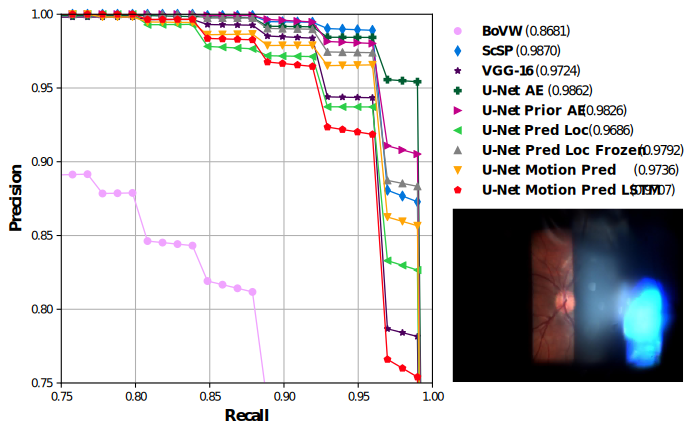
\includegraphics[width=12cm]{final_eval/ds14_pr}
  }
  \\[30pt]
  \subfloat[\textit{Max F1-Scores}]
  {
    \label{subfig:reprod_ds14}
    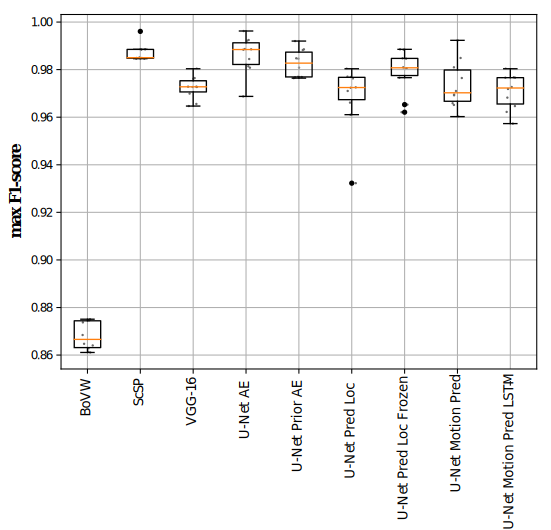
\includegraphics[width=10cm]{final_eval/ds14_reprod}
  }
  \caption{Detailed results on a \textit{Slitlamp} sequence. (a) \textit{PR-Curves} averaged on ten repetitions (b) Box-plot of \textit{max F1-Score} on each fold (median and standard deviation)}
  \label{fig:curves_ds14}  
\end{figure}

\clearpage
\begin{figure}[!htbp]
  \centering
  \subfloat[\textit{PR-Curves} of dataset \textit{MRI Brain B} with an example image]
  {
    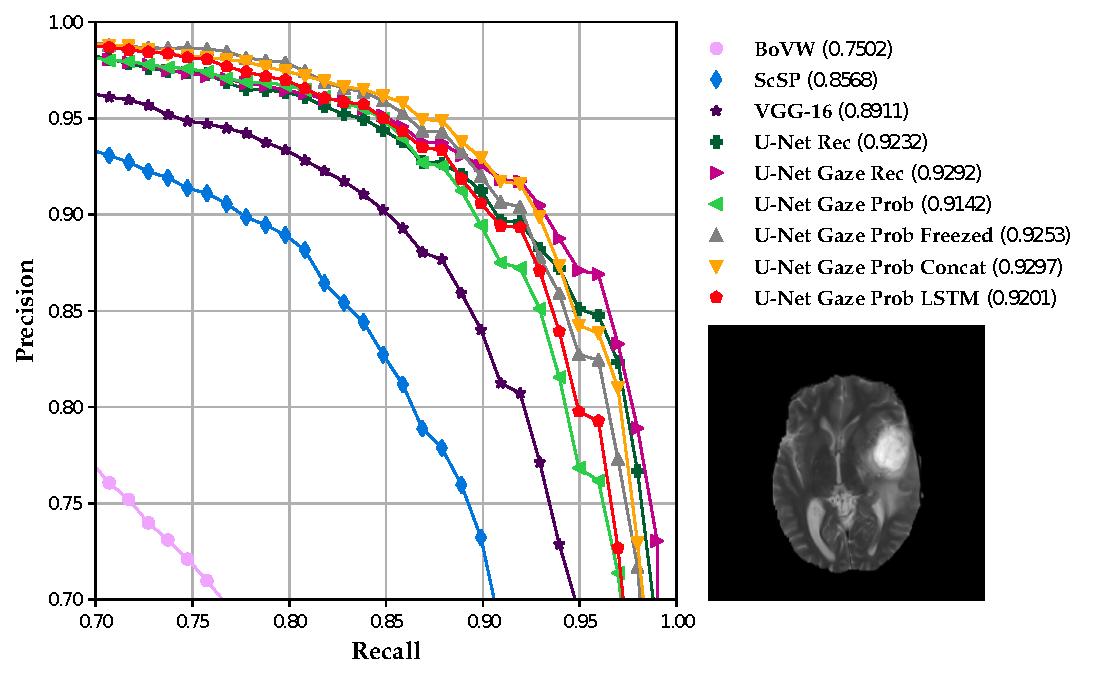
\includegraphics[width=12cm]{final_eval/ds16_pr}
  }
  \\[20pt]
  \subfloat[\textit{Max F1-Scores} of dataset \textit{MRI Brain B}]
  {
    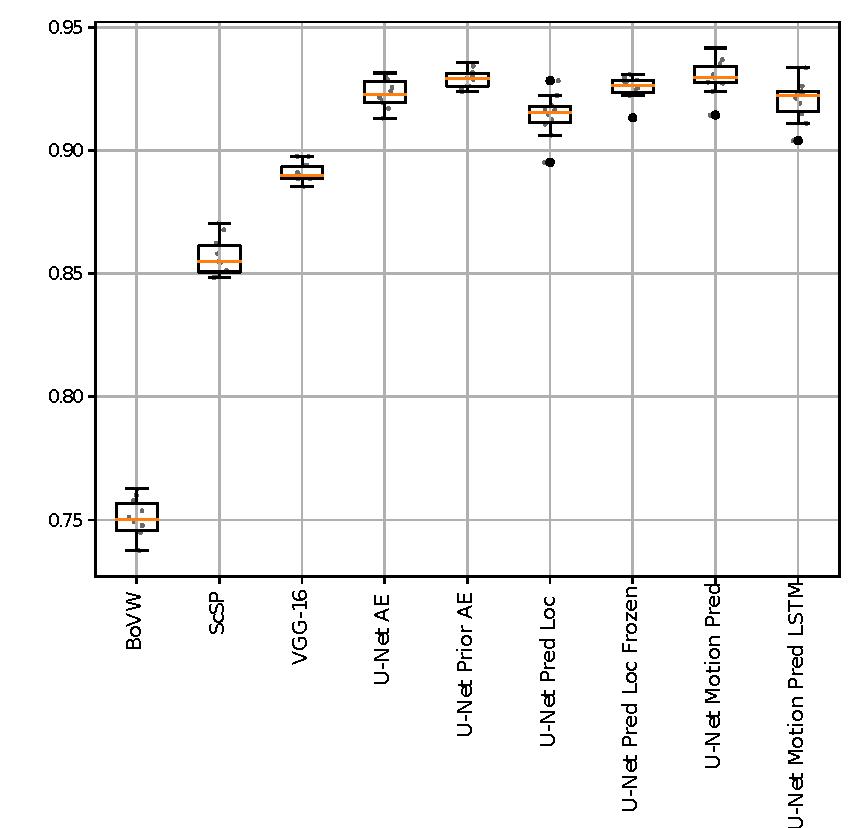
\includegraphics[width=10cm]{final_eval/ds16_reprod}
  }
  \caption{Detailed results on a \textit{Brain} sequence. (a) \textit{PR-Curves} averaged on ten repetitions. \textit{Max F1-Scores} are given in the legends. (b) Box-plot of \textit{max F1-Score} on each repetition (median and standard deviation).}
  \label{fig:curves_ds16}
\end{figure}


%%% Local Variables:
%%% mode: latex
%%% TeX-master: "../../main"
%%% End:
